\documentclass[12pt]{article}
\usepackage{amsmath}
\usepackage{amssymb}
\usepackage{graphicx}
\usepackage[margin=1in]{geometry}
\newcommand{\del}{\nabla}
\begin{document}

\title{Psych209 Final Project}
\author{Howon Lee}
\maketitle
\section*{Abstract}
%%% let's have the abstract last
\section*{Introduction}
\subsection*{Issue Addressed}

We wish to address the issue of using an alternative approach to introducing necessary non-determinism to the constraint satisfaction problem in a PDP system, as opposed to the Boltzmann machine with conventional simulated annealing.

An alternative optimization algorithm called $\tau$-extremal optimization($\tau$-EO) is used to update a constraint-satisfaction framework to escape local minima in short amounts of time. It, like simulated annealing, is inspired by condensed matter physics, but $\tau$-EO deals with nonequilibrium systems.

\subsection*{Why is it interesting?}

The update rule for Boltzmann machines in the general, non-restricted case is very powerful but not usable in practice. This is in part because of the enormous time needed to approach the network's equilibrium distribution. Therefore, other ways of avoiding local maxima and introducing nondeterminism in constraint satisfaction, besides simulated annealing of Boltzmann machines, might be of interest. Simulated annealing also has the disadvantage that it must be given an annealing schedule to work effectively, the proper tuning of which is extremely hard and problem-specific. Another source of interest is the possible exploration of the semantics of alternative ways to introduce nondeterminism into the constraint satisfaction framework in order to avoid the problem of local optima.

\subsection*{What has previously been done?}
%%% cite: extremal optimization, genetic algorithms
Extremal optimization, in general, is inspired by models of co-evolution. This is as opposed to genetic algorithms and evolutionary algorithms, which are inspired by evolution at a lower level of abstraction(per gene, not per species).

%%% cite: bak-sneppen, gould
To be specific, there exists a model of evolution called the Bak-Sneppen model, designed to bring about the time dynamics and other qualitative phenomena of evolution in the simplest method possible. It is a one-dimensional lattice model which models nothing about each species except its fitness and the structure of its relations with other species. $N$ species are considered as nodes on a graph which is a one-dimensional lattice (a ring), and each species has a fitness, denoted by a single scalar $\lambda$. At each discrete time step, the least fit species is replaced, and both of its neighbors replaced with it, with new species identical to the old ones except for the fitnesses, which are random. Notably, this selection organizes a fitness threshhold, below which species do not survive because they are always the least fit.

\begin{figure}
  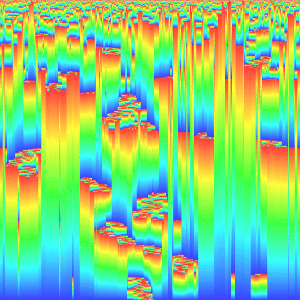
\includegraphics{bak_sneppen}
  %%% let's have a nice caption telling us stuff, citing the stuff.
\end{figure}

%%% cite Bak and Chialvo
One avenue of exploration was the adaptive extremal dynamics architecture promulgated by Bak and Chialvo as an alternative to conventional connectionist feedforward backpropagation neural nets. %%% what is it (what's the topology)? how does it work? explain why conjunctive neurons make it terribad, compare it to simulated annealing
\begin{figure}
  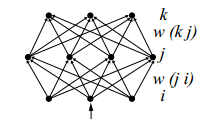
\includegraphics{bak_chialvo_net_topology}
\end{figure}
\begin{figure}
  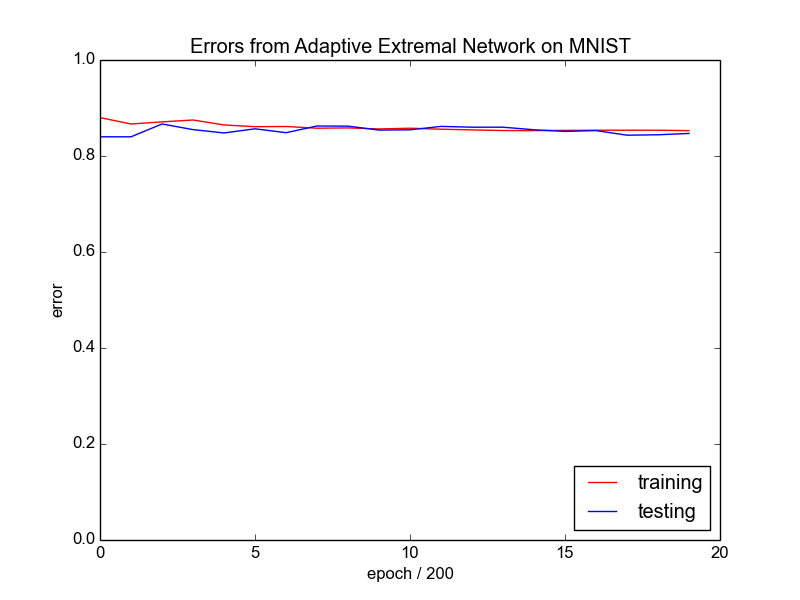
\includegraphics{bak_plot}
\end{figure}

%%% cite Boetticher
The model creates punctuated equilibrium because as the smallest fitness increases, it becomes more likely that the next smallest fitness is adjacent to the previous smallest fitness, and therefore the events become correlated, causing "avalanches". This behavior, if one considers the nodes in the graph to be variables in a problem instead of species, was noted to be desirable in optimization problems by Boettcher and Percus, and used as the basis of extremal optimization.

Extremal optimization can be described succinctly as iteratively identifying the worst performing variable (according to the variable's fitness, which the implementer must define) in a given solution and replacing them with a new component or swapping them out with another component. Since this is trivially subject to local optima(in fact, it is just a local search), this paper will mainly deal with a variant, $\tau$-extremal optimization, which solves this problem. It does so by ordering the local fitnesses, high to low, and choosing the $k$-ranked one, where

$$P(k) = Ck^{-\tau}$$

%%% cite the analytic claim that there's an optimum value of tau.
Where $C$ is a normalizing constant and $\tau$ is the one parameter. There is a claim by Boettcher et al that there is an analytically optimal value of $\tau$ for search time, which is $\tau = 1 + \frac{1}{\ln n}$, where $n$ is the number of variables.%%% by who??

%% cite the well-defined mean shit
The reason why the $P(k)$ is the way it is is because it gives an important advantage to the search pattern of $\tau$-extremal optimization: where other search algorithms are local or global, there is no well-defined scale to its search, because the $P(k)$ is a scale-free distribution, a power law which, because $\tau < 2$, does not have a well-defined mean or variance.

%%% cite hamming cliff
This solves an important problem called the \emph{Hamming cliff} in other evolution-inspired algorithms, where very many variables are coupled in a representation, such as in a conventional binary code, where the gap between 511 (0111111111) and 512 (1000000000) needs 10 coincident mutations. What would happen in the $\tau$-extremal optimization would be that the search would eventually perversely flip the first bit, and then proceed to quickly create an avalanche where it would flip all the other bits in the representation. Also because of this property, there does not need to be anything analogous to an annealing schedule for $\tau$-extremal optimization, where a more global search transforms into a more local search.

%%% cite TSP, graph cuts, ising models, hopfield net
The previous applications of EO and $\tau$-EO include the travelling salesman problem, graph cuts and Ising model spin glass optimization. It is the last of these that seems most important for us, because of the close connection between the Hopfield net and the Ising model, and in turn the Hopfield net and the constraint satisfaction networks that exist, including the Boltzmann machine, which can be construed as a probabilistic Hopfield net.

\begin{figure}
  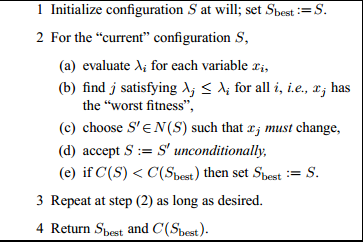
\includegraphics{eo_alg} %%%%% get a better pic
  \caption{extremal optimization algorithm}
\end{figure}


%%%% talk about replications HERE
%%%% talk about replications HERE
%%%% talk about replications HERE
%%%% talk about replications HERE
  \frametitle{Ising Model}
  \begin{figure}
    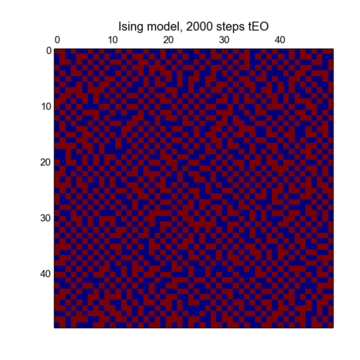
\includegraphics{2000}
  \end{figure}
  \begin{figure}
    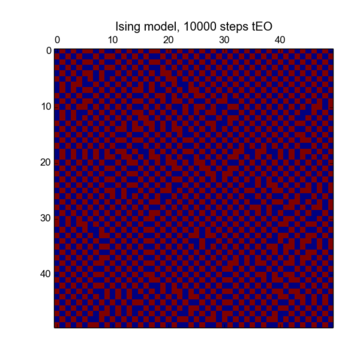
\includegraphics{10000}
  \end{figure}
  \begin{figure}
    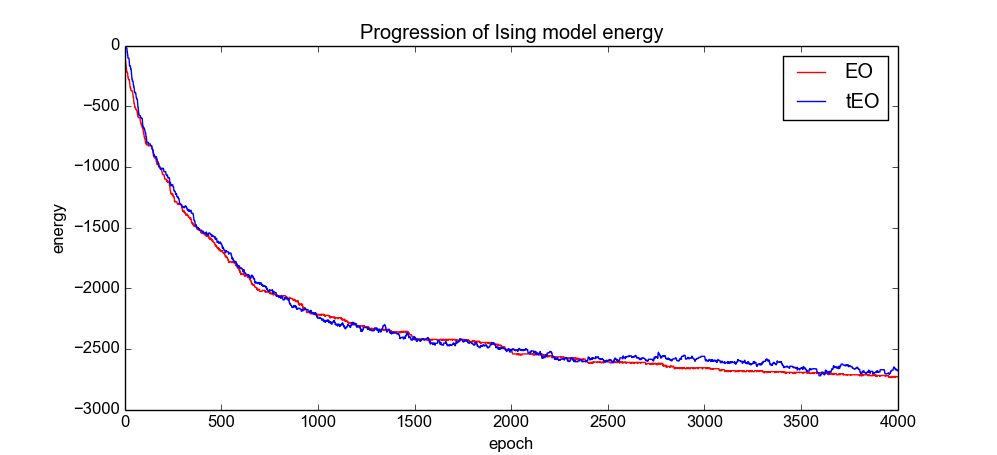
\includegraphics{ising_energy_unzoomed}
  \end{figure}
  
  \begin{figure}
    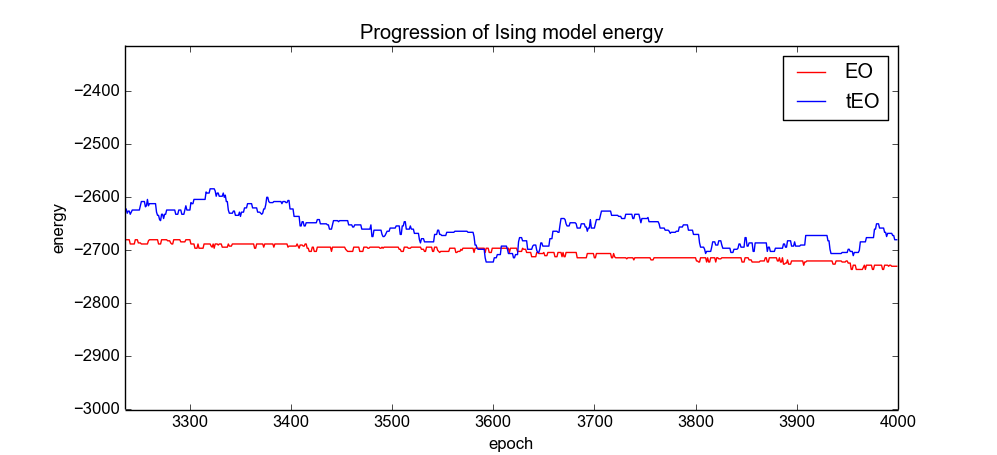
\includegraphics{ising_energy_zoomed}
  \end{figure}
  
\section{Novel Approach}

%%%%% moar pictures, figures, shit like that

%%% cite schema network
Because of the problem of long simulation times of the Boltzmann machine and of the close relation of the Boltzmann machine to the Ising models which had already been simulated in the literature, a constraint satisfaction network was made which would have non-determinimism introduced to it by using the $\tau$-EO algorithm, just as a Boltzmann machine can be construed as a schema network with non-determinism introduced into it in another way.

%%% cite boettcher et al for the optimum of tau
In order to do this, we needed to choose a $\tau$ and to determine the fitness function. Both are fairly obvious: we chose the claimed analytic optimum from Boetcher et al and we chose the already existing goodness function from the PDP version of the schema network.

% cite rbm
In addition, we had a preliminary investigation into trying to use the $\tau$-extremal optimization into learning. Because we were investigating learning only, we decided to use a more commonly used constraint satisfier, the restricted Boltzmann machine, and then to use the more commonly used contrastive divergence to estimate the equilibrium distribution. The \emph{gradients} in this case were treated as the fitnesses, making this algorithm a sort of adaptive line search.

\section{Details of Approach}

%%% rbm try learning mechanism, a sort of gradient descent. still try contrastive divergence in order to get the gradient in the first place. note the differentiation between the fitness as the _gradient_, which applies here, and the fitness as the _energy_, which applies to our one successful experiment.

%%% going to note the fact that I did bm normally now
% for the csp:
%We want to do speed.
% we also have a feeling that there's going to be a skewed distribution of speeds: that is, there's going to be a lot of cases where we're perilously close to a local optima
% therefore, we actually want to explore the entire possible initial activation space of a problem. that's not going to happen with a 'real' problem like MNIST, so we did the Necker cube problem from PDP
% simulation of the report only, since in this case the learning algorithm would actually be almost the same: note the failure of the extremal algrithm to produce extremal behavior in the learning case
% will graph time

%Specific target phenomenon or phenomena you will be addressing: e.g., pattern of data you intend to try to fit. Model network task setting, architecture, processing and learning algorithm, training environment (corpus used for training, knowledge base built in to network),


\section{Results and Analysis}
%%First present your primary findings that bear directly on the target phenomena.
%%% it's faster
  
\begin{figure}
    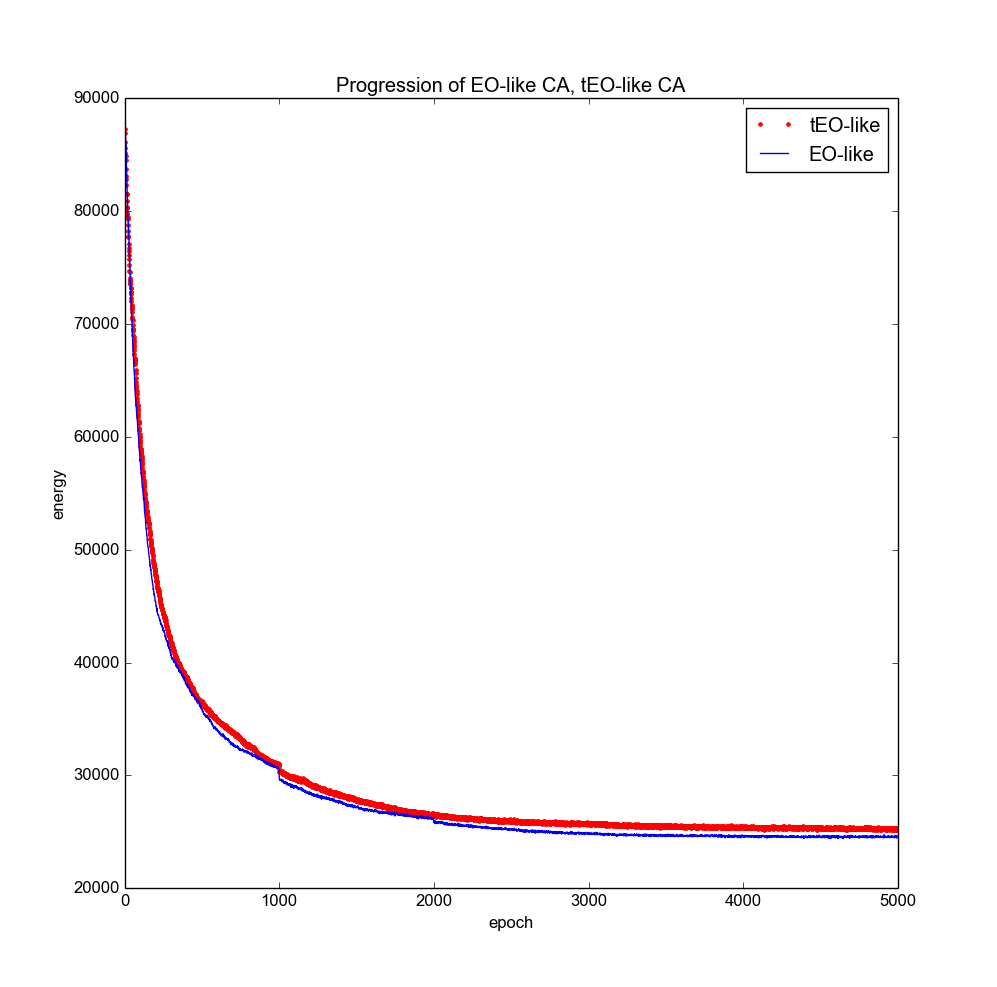
\includegraphics{eo_rbm_unzoomed}
  \end{figure}
  %%%%% spiffy speed figure

%%A strong paper will, in addition, present an analysis of why the results came out the way they did, especially in cases where results did not come out as expected. 
%%% why is it faster?
%%% note the fasterness of SA compared to schedule SA is partly an artifact of the fact that we demand a global minima: the schedule tends to get stuck in local minima
%%% but why is the tauEO faster? immediately after it makes a huge jump to escape local minima, the power law distribution of tau means that it will tend to explore the new local state space really fast, for basically the same reason that it's an online algorithm.
%% work an example of the local maxima escape, audacious courage, extremistan

%%It can be useful to discuss results you obtain with one of us to get suggestions as to how to fully understand your findings.

%%Analysis not only of network outputs but also of the structure of the information present in the materials you use to train your network (when relevant) and / or the hidden unit activations, network weights, or learning trajectory can help illuminate why and how your network has performed the way it did.

\section{Discussion}

It must be noted that, unlike simulated annealing with an annealing schedule, which doesn't work as an online algorithm, or an algorithm which can be given its input piece by piece, that there is nothing preventing $\tau$-extremal optimization from being used online.

%%% cite Boettcher for the disequilibrium stuff
The theoretical basis for the difference 

%%% theoretincal thoughts: out of equilibrium
%%% theoretical thoughts: black magic in determining the number of iterations, very associated with the fact of being an online algorithm

%Summarize your goals, your approach, and your main findings, and state a conclusion indicating how well, overall, your goals have been met.

%%% goals: make a faster thing than SA for abstract csp
%%% approach: tau-EO for cs net
%%% findings: spiffy results
%Then, discuss shortcomings or limitations of your effort and indicate how these might be overcome in future work.
%%% limitations: limited net, not fully connected, not a real problem. doesn't scale up.
%%% limitations: not thinking hard about neuronal connectivity. one thing that continues on the subject of criticality is modelling chialvo's work
%%% broader implications: try to look carefully at the critical regions of abstract NP-complete problem
%%Also, indicate broader implications and potential future applications of the ideas and approach.

\subsection*{What remains to be done?}
Because this project attempted to completely explore an entire state space of a problem, it was not feasible to explore a non-toy problem: that is, a problem where it's not possible to explore the entire state space, and therefore other measures of speech must be checked. It remains to be seen if this speed can be replicated in a larger problem domain with different local optima.

%%% cite chialvo
%%% compare to Chialvo stuff
It cannot necessarily be the case that a power law is evidence for \emph{only} self-organized criticality, but %%begin and finish this

\section{Summary}

Citations:   We will not be sticklers for details of citation styles but do provide citations to literature you draw on in your paper, using the following format

\end{document}

